% Created by tikzDevice version 0.12.6 on 2026-08-08 12:11:48
% !TEX encoding = UTF-8 Unicode
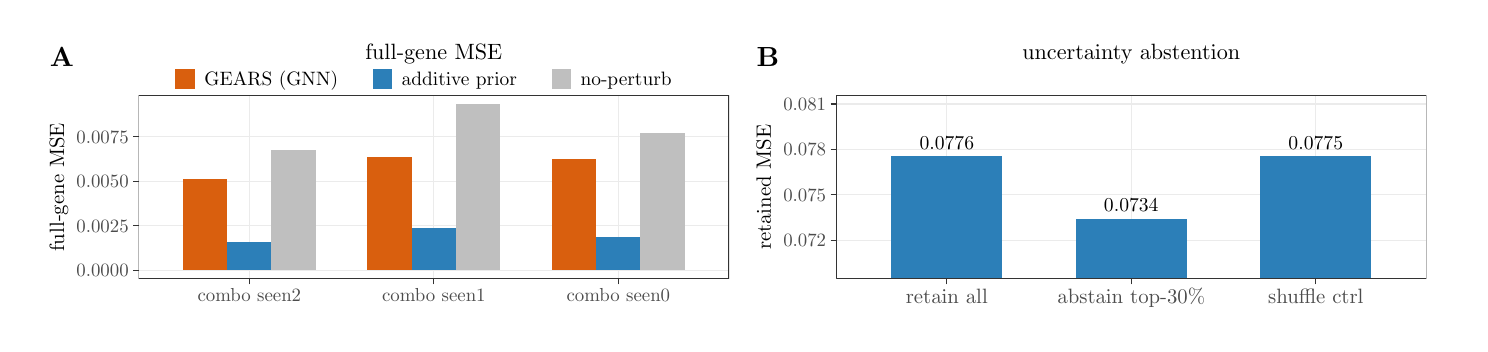
\begin{tikzpicture}[x=1pt,y=1pt]
\definecolor{fillColor}{RGB}{255,255,255}
\path[use as bounding box,fill=fillColor,fill opacity=0.00] (0,0) rectangle (517.45,106.96);
\begin{scope}
\path[clip] (  0.00,  0.00) rectangle (517.45,106.96);
\definecolor{drawColor}{RGB}{255,255,255}
\definecolor{fillColor}{RGB}{255,255,255}

\path[draw=drawColor,line width= 0.4pt,line join=round,line cap=round,fill=fillColor] ( -0.00,  0.00) rectangle (517.45,106.96);
\end{scope}
\begin{scope}
\path[clip] (  4.00,  3.00) rectangle (259.43,103.96);
\definecolor{drawColor}{RGB}{255,255,255}
\definecolor{fillColor}{RGB}{255,255,255}

\path[draw=drawColor,line width= 0.4pt,line join=round,line cap=round,fill=fillColor] (  4.00,  3.00) rectangle (259.43,103.96);
\end{scope}
\begin{scope}
\path[clip] (259.43,  3.00) rectangle (511.45,103.96);
\definecolor{drawColor}{RGB}{255,255,255}
\definecolor{fillColor}{RGB}{255,255,255}

\path[draw=drawColor,line width= 0.4pt,line join=round,line cap=round,fill=fillColor] (259.43,  3.00) rectangle (511.45,103.96);
\end{scope}
\begin{scope}
\path[clip] ( 40.11, 16.22) rectangle (253.43, 82.39);
\definecolor{fillColor}{RGB}{255,255,255}

\path[fill=fillColor] ( 40.11, 16.22) rectangle (253.43, 82.39);
\definecolor{drawColor}{gray}{0.92}

\path[draw=drawColor,line width= 0.4pt,line join=round] ( 40.11, 19.23) --
	(253.43, 19.23);

\path[draw=drawColor,line width= 0.4pt,line join=round] ( 40.11, 35.33) --
	(253.43, 35.33);

\path[draw=drawColor,line width= 0.4pt,line join=round] ( 40.11, 51.43) --
	(253.43, 51.43);

\path[draw=drawColor,line width= 0.4pt,line join=round] ( 40.11, 67.54) --
	(253.43, 67.54);

\path[draw=drawColor,line width= 0.4pt,line join=round] ( 80.10, 16.22) --
	( 80.10, 82.39);

\path[draw=drawColor,line width= 0.4pt,line join=round] (146.77, 16.22) --
	(146.77, 82.39);

\path[draw=drawColor,line width= 0.4pt,line join=round] (213.43, 16.22) --
	(213.43, 82.39);
\definecolor{fillColor}{RGB}{217,95,14}

\path[fill=fillColor] ( 56.11, 19.23) rectangle ( 72.11, 52.34);
\definecolor{fillColor}{RGB}{44,127,184}

\path[fill=fillColor] ( 72.11, 19.23) rectangle ( 88.10, 29.47);
\definecolor{fillColor}{gray}{0.75}

\path[fill=fillColor] ( 88.10, 19.23) rectangle (104.10, 62.64);
\definecolor{fillColor}{RGB}{217,95,14}

\path[fill=fillColor] (122.77, 19.23) rectangle (138.77, 60.19);
\definecolor{fillColor}{RGB}{44,127,184}

\path[fill=fillColor] (138.77, 19.23) rectangle (154.77, 34.62);
\definecolor{fillColor}{gray}{0.75}

\path[fill=fillColor] (154.77, 19.23) rectangle (170.77, 79.39);
\definecolor{fillColor}{RGB}{217,95,14}

\path[fill=fillColor] (189.43, 19.23) rectangle (205.43, 59.36);
\definecolor{fillColor}{RGB}{44,127,184}

\path[fill=fillColor] (205.43, 19.23) rectangle (221.43, 31.47);
\definecolor{fillColor}{gray}{0.75}

\path[fill=fillColor] (221.43, 19.23) rectangle (237.43, 69.08);
\definecolor{drawColor}{gray}{0.20}

\path[draw=drawColor,line width= 0.4pt,line join=round,line cap=round] ( 40.11, 16.22) rectangle (253.43, 82.39);
\end{scope}
\begin{scope}
\path[clip] (  0.00,  0.00) rectangle (517.45,106.96);
\definecolor{drawColor}{gray}{0.30}

\node[text=drawColor,anchor=base east,inner sep=0pt, outer sep=0pt, scale=  0.68] at ( 36.51, 16.89) {0.0000};

\node[text=drawColor,anchor=base east,inner sep=0pt, outer sep=0pt, scale=  0.68] at ( 36.51, 32.99) {0.0025};

\node[text=drawColor,anchor=base east,inner sep=0pt, outer sep=0pt, scale=  0.68] at ( 36.51, 49.09) {0.0050};

\node[text=drawColor,anchor=base east,inner sep=0pt, outer sep=0pt, scale=  0.68] at ( 36.51, 65.19) {0.0075};
\end{scope}
\begin{scope}
\path[clip] (  0.00,  0.00) rectangle (517.45,106.96);
\definecolor{drawColor}{gray}{0.20}

\path[draw=drawColor,line width= 0.4pt,line join=round] ( 38.11, 19.23) --
	( 40.11, 19.23);

\path[draw=drawColor,line width= 0.4pt,line join=round] ( 38.11, 35.33) --
	( 40.11, 35.33);

\path[draw=drawColor,line width= 0.4pt,line join=round] ( 38.11, 51.43) --
	( 40.11, 51.43);

\path[draw=drawColor,line width= 0.4pt,line join=round] ( 38.11, 67.54) --
	( 40.11, 67.54);
\end{scope}
\begin{scope}
\path[clip] (  0.00,  0.00) rectangle (517.45,106.96);
\definecolor{drawColor}{gray}{0.20}

\path[draw=drawColor,line width= 0.4pt,line join=round] ( 80.10, 14.22) --
	( 80.10, 16.22);

\path[draw=drawColor,line width= 0.4pt,line join=round] (146.77, 14.22) --
	(146.77, 16.22);

\path[draw=drawColor,line width= 0.4pt,line join=round] (213.43, 14.22) --
	(213.43, 16.22);
\end{scope}
\begin{scope}
\path[clip] (  0.00,  0.00) rectangle (517.45,106.96);
\definecolor{drawColor}{gray}{0.30}

\node[text=drawColor,anchor=base,inner sep=0pt, outer sep=0pt, scale=  0.68] at ( 80.10,  7.94) {combo seen2};

\node[text=drawColor,anchor=base,inner sep=0pt, outer sep=0pt, scale=  0.68] at (146.77,  7.94) {combo seen1};

\node[text=drawColor,anchor=base,inner sep=0pt, outer sep=0pt, scale=  0.68] at (213.43,  7.94) {combo seen0};
\end{scope}
\begin{scope}
\path[clip] (  0.00,  0.00) rectangle (517.45,106.96);
\definecolor{drawColor}{RGB}{0,0,0}

\node[text=drawColor,rotate= 90.00,anchor=base,inner sep=0pt, outer sep=0pt, scale=  0.75] at ( 13.17, 49.31) {full-gene MSE};
\end{scope}
\begin{scope}
\path[clip] (  0.00,  0.00) rectangle (517.45,106.96);
\definecolor{fillColor}{RGB}{255,255,255}

\path[fill=fillColor] ( 51.85, 84.39) rectangle (241.69, 92.39);
\end{scope}
\begin{scope}
\path[clip] (  0.00,  0.00) rectangle (517.45,106.96);
\definecolor{fillColor}{RGB}{255,255,255}

\path[fill=fillColor] ( 52.85, 84.39) rectangle ( 60.85, 92.39);
\definecolor{fillColor}{RGB}{217,95,14}

\path[fill=fillColor] ( 53.36, 84.91) rectangle ( 60.33, 91.88);
\end{scope}
\begin{scope}
\path[clip] (  0.00,  0.00) rectangle (517.45,106.96);
\definecolor{fillColor}{RGB}{255,255,255}

\path[fill=fillColor] (124.15, 84.39) rectangle (132.15, 92.39);
\definecolor{fillColor}{RGB}{44,127,184}

\path[fill=fillColor] (124.67, 84.91) rectangle (131.64, 91.88);
\end{scope}
\begin{scope}
\path[clip] (  0.00,  0.00) rectangle (517.45,106.96);
\definecolor{fillColor}{RGB}{255,255,255}

\path[fill=fillColor] (188.79, 84.39) rectangle (196.79, 92.39);
\definecolor{fillColor}{gray}{0.75}

\path[fill=fillColor] (189.31, 84.91) rectangle (196.28, 91.88);
\end{scope}
\begin{scope}
\path[clip] (  0.00,  0.00) rectangle (517.45,106.96);
\definecolor{drawColor}{RGB}{0,0,0}

\node[text=drawColor,anchor=base west,inner sep=0pt, outer sep=0pt, scale=  0.70] at ( 63.85, 85.98) {GEARS (GNN)};
\end{scope}
\begin{scope}
\path[clip] (  0.00,  0.00) rectangle (517.45,106.96);
\definecolor{drawColor}{RGB}{0,0,0}

\node[text=drawColor,anchor=base west,inner sep=0pt, outer sep=0pt, scale=  0.70] at (135.15, 85.98) {additive prior};
\end{scope}
\begin{scope}
\path[clip] (  0.00,  0.00) rectangle (517.45,106.96);
\definecolor{drawColor}{RGB}{0,0,0}

\node[text=drawColor,anchor=base west,inner sep=0pt, outer sep=0pt, scale=  0.70] at (199.79, 85.98) {no-perturb};
\end{scope}
\begin{scope}
\path[clip] (  0.00,  0.00) rectangle (517.45,106.96);
\definecolor{drawColor}{RGB}{0,0,0}

\node[text=drawColor,anchor=base,inner sep=0pt, outer sep=0pt, scale=  0.80] at (146.77, 95.45) {full-gene MSE};
\end{scope}
\begin{scope}
\path[clip] (  0.00,  0.00) rectangle (517.45,106.96);
\definecolor{drawColor}{RGB}{0,0,0}

\node[text=drawColor,anchor=base,inner sep=0pt, outer sep=0pt, scale=  1.00] at ( 12.35, 93.09) {\bfseries A};
\end{scope}
\begin{scope}
\path[clip] (292.13, 16.22) rectangle (505.45, 82.39);
\definecolor{fillColor}{RGB}{255,255,255}

\path[fill=fillColor] (292.13, 16.22) rectangle (505.45, 82.39);
\definecolor{drawColor}{gray}{0.92}

\path[draw=drawColor,line width= 0.4pt,line join=round] (292.13, 30.17) --
	(505.45, 30.17);

\path[draw=drawColor,line width= 0.4pt,line join=round] (292.13, 46.57) --
	(505.45, 46.57);

\path[draw=drawColor,line width= 0.4pt,line join=round] (292.13, 62.98) --
	(505.45, 62.98);

\path[draw=drawColor,line width= 0.4pt,line join=round] (292.13, 79.39) --
	(505.45, 79.39);

\path[draw=drawColor,line width= 0.4pt,line join=round] (332.13, 16.22) --
	(332.13, 82.39);

\path[draw=drawColor,line width= 0.4pt,line join=round] (398.79, 16.22) --
	(398.79, 82.39);

\path[draw=drawColor,line width= 0.4pt,line join=round] (465.46, 16.22) --
	(465.46, 82.39);
\definecolor{fillColor}{RGB}{44,127,184}

\path[fill=fillColor] (312.13,-363.58) rectangle (352.13, 60.57);

\path[fill=fillColor] (378.80,-363.58) rectangle (418.79, 37.99);

\path[fill=fillColor] (445.46,-363.58) rectangle (485.45, 60.41);
\definecolor{drawColor}{RGB}{0,0,0}

\node[text=drawColor,anchor=base,inner sep=0pt, outer sep=0pt, scale=  0.71] at (332.13, 63.02) {0.0776};

\node[text=drawColor,anchor=base,inner sep=0pt, outer sep=0pt, scale=  0.71] at (398.79, 40.44) {0.0734};

\node[text=drawColor,anchor=base,inner sep=0pt, outer sep=0pt, scale=  0.71] at (465.46, 62.86) {0.0775};
\definecolor{drawColor}{gray}{0.20}

\path[draw=drawColor,line width= 0.4pt,line join=round,line cap=round] (292.13, 16.22) rectangle (505.45, 82.39);
\end{scope}
\begin{scope}
\path[clip] (  0.00,  0.00) rectangle (517.45,106.96);
\definecolor{drawColor}{gray}{0.30}

\node[text=drawColor,anchor=base east,inner sep=0pt, outer sep=0pt, scale=  0.68] at (288.53, 27.83) {0.072};

\node[text=drawColor,anchor=base east,inner sep=0pt, outer sep=0pt, scale=  0.68] at (288.53, 44.23) {0.075};

\node[text=drawColor,anchor=base east,inner sep=0pt, outer sep=0pt, scale=  0.68] at (288.53, 60.64) {0.078};

\node[text=drawColor,anchor=base east,inner sep=0pt, outer sep=0pt, scale=  0.68] at (288.53, 77.05) {0.081};
\end{scope}
\begin{scope}
\path[clip] (  0.00,  0.00) rectangle (517.45,106.96);
\definecolor{drawColor}{gray}{0.20}

\path[draw=drawColor,line width= 0.4pt,line join=round] (290.13, 30.17) --
	(292.13, 30.17);

\path[draw=drawColor,line width= 0.4pt,line join=round] (290.13, 46.57) --
	(292.13, 46.57);

\path[draw=drawColor,line width= 0.4pt,line join=round] (290.13, 62.98) --
	(292.13, 62.98);

\path[draw=drawColor,line width= 0.4pt,line join=round] (290.13, 79.39) --
	(292.13, 79.39);
\end{scope}
\begin{scope}
\path[clip] (  0.00,  0.00) rectangle (517.45,106.96);
\definecolor{drawColor}{gray}{0.20}

\path[draw=drawColor,line width= 0.4pt,line join=round] (332.13, 14.22) --
	(332.13, 16.22);

\path[draw=drawColor,line width= 0.4pt,line join=round] (398.79, 14.22) --
	(398.79, 16.22);

\path[draw=drawColor,line width= 0.4pt,line join=round] (465.46, 14.22) --
	(465.46, 16.22);
\end{scope}
\begin{scope}
\path[clip] (  0.00,  0.00) rectangle (517.45,106.96);
\definecolor{drawColor}{gray}{0.30}

\node[text=drawColor,anchor=base,inner sep=0pt, outer sep=0pt, scale=  0.75] at (332.13,  7.46) {retain all};

\node[text=drawColor,anchor=base,inner sep=0pt, outer sep=0pt, scale=  0.75] at (398.79,  7.46) {abstain top-30\%};

\node[text=drawColor,anchor=base,inner sep=0pt, outer sep=0pt, scale=  0.75] at (465.46,  7.46) {shuffle ctrl};
\end{scope}
\begin{scope}
\path[clip] (  0.00,  0.00) rectangle (517.45,106.96);
\definecolor{drawColor}{RGB}{0,0,0}

\node[text=drawColor,rotate= 90.00,anchor=base,inner sep=0pt, outer sep=0pt, scale=  0.75] at (268.59, 49.31) {retained MSE};
\end{scope}
\begin{scope}
\path[clip] (  0.00,  0.00) rectangle (517.45,106.96);
\definecolor{drawColor}{RGB}{0,0,0}

\node[text=drawColor,anchor=base,inner sep=0pt, outer sep=0pt, scale=  0.80] at (398.79, 95.45) {uncertainty abstention};
\end{scope}
\begin{scope}
\path[clip] (  0.00,  0.00) rectangle (517.45,106.96);
\definecolor{drawColor}{RGB}{0,0,0}

\node[text=drawColor,anchor=base,inner sep=0pt, outer sep=0pt, scale=  1.00] at (267.52, 93.09) {\bfseries B};
\end{scope}
\end{tikzpicture}
